%\subsection{Eigenspace Overlap}
%\label{subsec:eigen_overlap}
%	\begin{itemize}
%		\item Introduce the eigenspace overlap metric.
%%		\item Present the generalization bound.
%	\end{itemize}
%	
%\subsection{Generalization of Compressed Embeddings}
%\label{subsec:revisit}
%	\begin{itemize}
%		\item Empirically demonstrate the correlation with respect to generalization performance
%		\item Discuss why it explains better than Deltas (if have not discuss the relation to Deltas, we should discuss here also).
%	\end{itemize}

\begin{table*}
	\caption{The Spearman rank correlation coefficient $\rho$ between compression quality metrics and downstream performance. The larger the absolute value of the coefficient, the stronger the correlation is.
	Within each entry in the table, the correlations are presented in terms of `GloVe (Wiki'14) $\rho$ \;/\; GloVe (Wiki'17) $\rho$ \;/\; fastText $\rho$'.
	}
	\small
	\begin{tabular}{c | c | c | c | c}
		\toprule
		& QA & Sentiment & Analogy & Similarity \\
		\midrule
		Embed. reconst. error &  $-0.61/-0.22/-0.84$  &  $-0.40/-0.25/-0.69$  &  $\mathbf{-0.98/-1.00}/-0.88$  &  $-0.19/0.77/-0.36$  \\ 
		PIP loss &  $-0.49/-0.32/-0.74$  &  $-0.29/-0.27/-0.61$  &  $-0.82/-0.67/-0.82$  &  $0.05/-0.07/-0.23$  \\  
		$1/(1-\Delta_1)$ &  $-0.62/-0.83/-0.77$  &  $-0.42/-0.79/-0.56$  &  $-0.90/-0.98/-0.90$  &  $-0.22/-0.69/-0.31$  \\  
		$\Delta_2$ &  $-0.46/-0.87/0.18$  &  $-0.39/-0.87/0.30$  &  $-0.70/-0.82/-0.02$  &  $-0.43/-0.72/-0.15$  \\  
		$1 - \mathcal{E}$ & $\mathbf{-0.81/-0.97/-0.90}$  &  $\mathbf{-0.72/-0.96/-0.73}$  &  $-0.79/-0.91/\mathbf{-0.96}$  &  $\mathbf{-0.62/-0.88/-0.67}$  \\  
		%%	\midrule
		%Embed. reconst. error & & & & \\
		%%	\midrule
		%PIP loss & & & & \\
		%%	\midrule
		%$1/(1-\Delta_1)$ & & & & \\
		%%	\midrule
		%$\Delta_2$ & & & & \\
		%%	\midrule
		%$\mathcal{E}$ & & & & \\
		\bottomrule
	\end{tabular}
	\label{tab:sp_rank}
\end{table*}

%\begin{figure*}
%	\footnotesize
%	\begin{tabular}{@{\hskip -0.0in}c@{\hskip -0.0in}c@{\hskip -0.0in}c@{\hskip -0.0in}c@{\hskip -0.0in}}
%		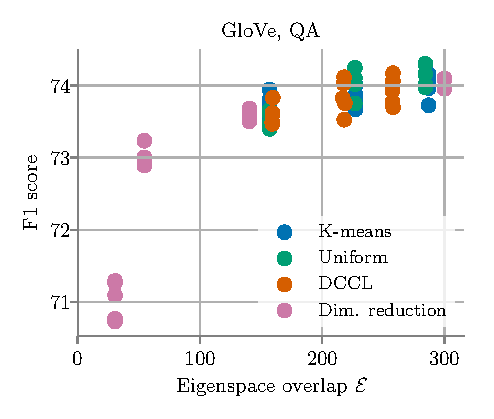
\includegraphics[width=.245\linewidth]{figures/glove400k_qa_best-f1_vs_subspace-eig-overlap_linx.pdf} &
%		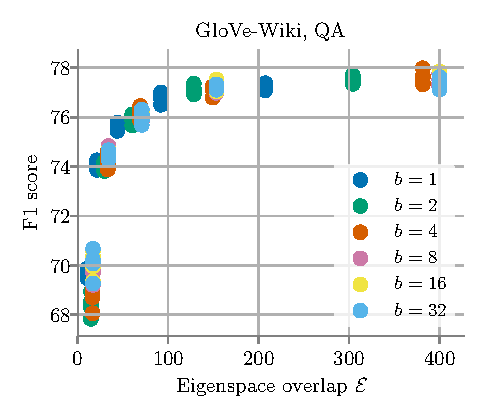
\includegraphics[width=.245\linewidth]{figures/glove-wiki400k-am_qa_best-f1_vs_subspace-eig-overlap_linx.pdf} &
%		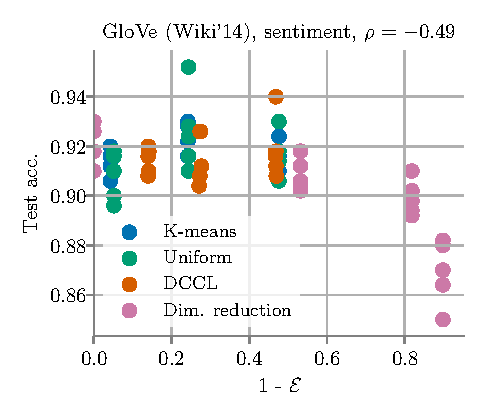
\includegraphics[width=.245\linewidth]{figures/glove400k_sentiment_trec_test-acc_vs_subspace-eig-overlap_linx.pdf} &
%		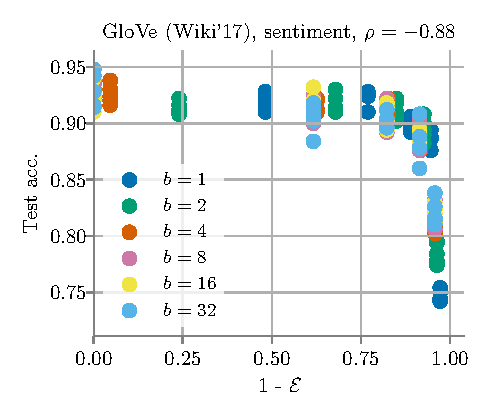
\includegraphics[width=.245\linewidth]{figures/glove-wiki400k-am_sentiment_trec_test-acc_vs_subspace-eig-overlap_linx.pdf}	\\
%		(a) GloVe (Wiki'14), QA & \;\;\;\;(b) GloVe (Wiki'17), QA  & \;\;\;\;\;\;(c) GloVe (Wiki'14), sentiment & \;\;\;\;\;(d) GloVe (Wiki'14)
%	\end{tabular}
%	\caption{Our proposed compression quality metric eigenspace overlap correlates strongly with the downstream task performance of compressed embeddings.  On both the question answering and sentiment analysis task, we demonstrate that eigenspace overlap consistently achieves strong correlation 1) across different compression methods (shown in (a), (c)) and 2) across different precision for the uniform quantization methods (shown in (b), (d)). In other words, embeddings compressed by different methods using different configurations can performs similarly in downstream tasks, when they have similar eigenspace overlap with the same reference uncompressed embedding.}
%	\label{fig:good_correlation}
%\end{figure*}

\begin{figure*}
	\footnotesize
	\begin{tabular}{@{\hskip -0.0in}c@{\hskip -0.0in}c@{\hskip -0.0in}c@{\hskip -0.0in}c@{\hskip -0.0in}}
		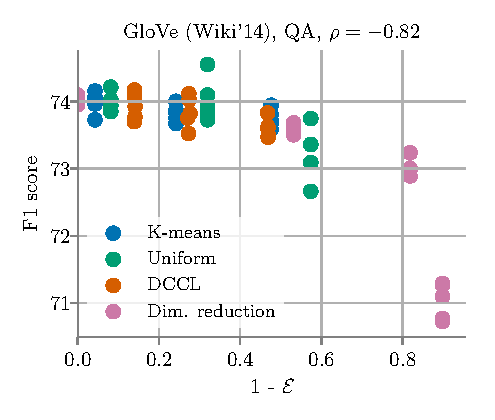
\includegraphics[width=.245\linewidth]{figures/glove400k_qa_best-f1_vs_subspace-dist-normalized_linx_stoc.pdf} &
		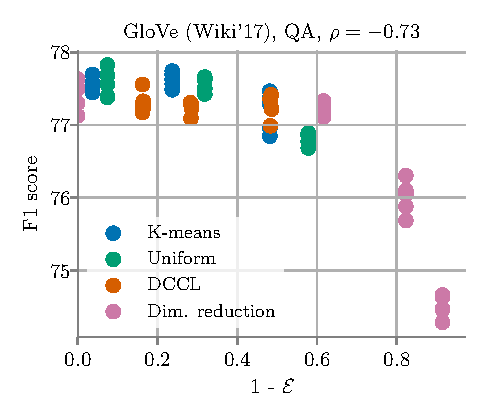
\includegraphics[width=.245\linewidth]{figures/glove-wiki400k-am_qa_best-f1_vs_subspace-dist-normalized_linx_stoc.pdf} &
		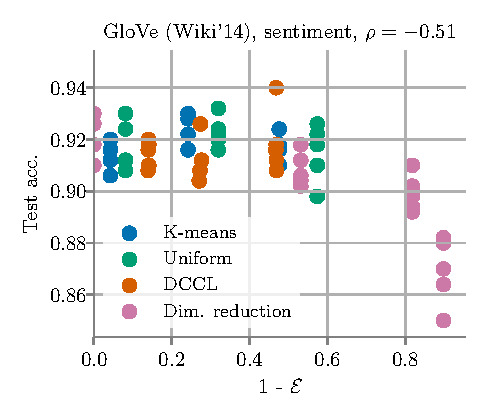
\includegraphics[width=.245\linewidth]{figures/glove400k_sentiment_trec_test-acc_vs_subspace-dist-normalized_linx_stoc.pdf} &
		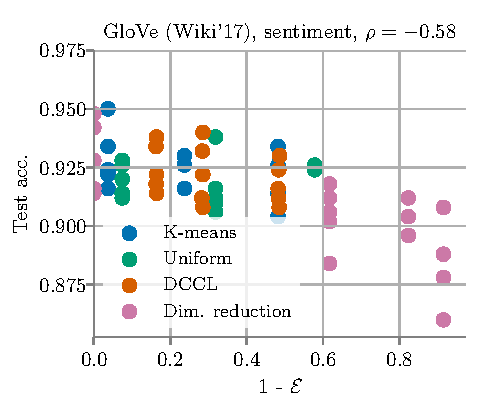
\includegraphics[width=.245\linewidth]{figures/glove-wiki400k-am_sentiment_trec_test-acc_vs_subspace-dist-normalized_linx_stoc.pdf}	\\
		(a) GloVe (Wiki'14), QA & \;\;\;\;(b) GloVe (Wiki'17), QA  & \;\;\;\;\;\;(c) GloVe (Wiki'14), sentiment & \;\;\;\;\;(d) GloVe (Wiki'14)
	\end{tabular}
	\caption{\textbf{Stochastic.} Our proposed compression quality metric eigenspace overlap correlates strongly with the downstream task performance of compressed embeddings.  On both the question answering and sentiment analysis task, we demonstrate that eigenspace overlap consistently achieves strong correlation 1) across different compression methods (shown in (a), (c)) and 2) across different precision for the uniform quantization methods (shown in (b), (d)). In other words, embeddings compressed by different methods using different configurations can performs similarly in downstream tasks, when they have similar eigenspace overlap with the same reference uncompressed embedding.}
	\label{fig:good_correlation_stoc}
\end{figure*}

\begin{figure*}
	\footnotesize
	\begin{tabular}{@{\hskip -0.0in}c@{\hskip -0.0in}c@{\hskip -0.0in}c@{\hskip -0.0in}c@{\hskip -0.0in}}
		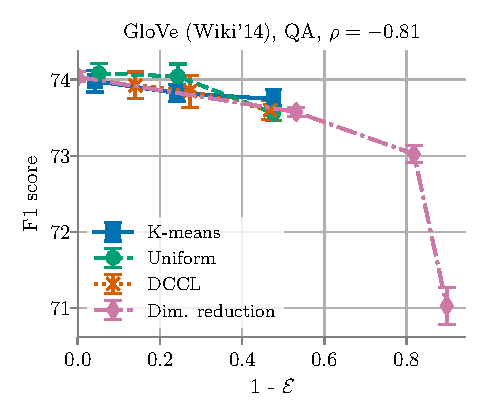
\includegraphics[width=.245\linewidth]{figures/glove400k_qa_best-f1_vs_subspace-dist-normalized_linx_det.pdf} &
		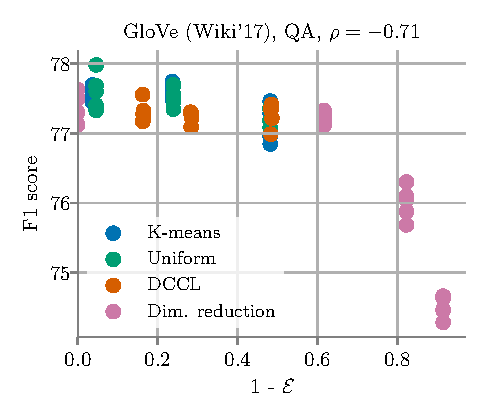
\includegraphics[width=.245\linewidth]{figures/glove-wiki400k-am_qa_best-f1_vs_subspace-dist-normalized_linx_det.pdf} &
		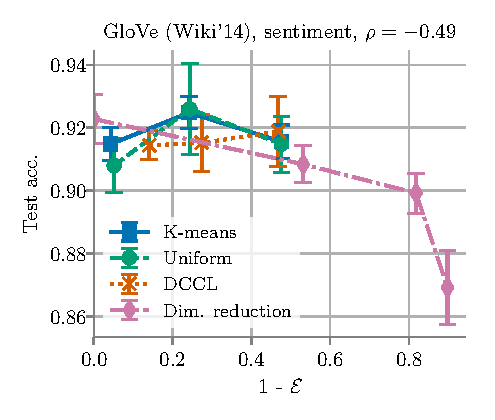
\includegraphics[width=.245\linewidth]{figures/glove400k_sentiment_trec_test-acc_vs_subspace-dist-normalized_linx_det.pdf} &
		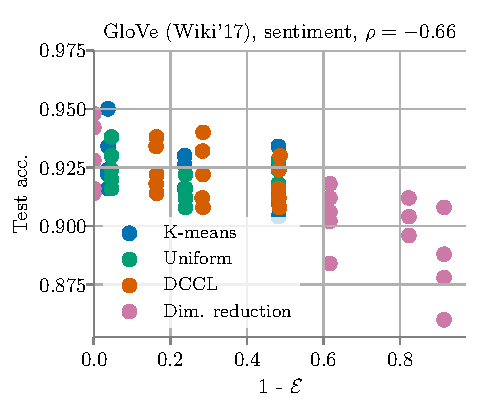
\includegraphics[width=.245\linewidth]{figures/glove-wiki400k-am_sentiment_trec_test-acc_vs_subspace-dist-normalized_linx_det.pdf}	\\
		(a) GloVe (Wiki'14), QA & \;\;\;\;(b) GloVe (Wiki'17), QA  & \;\;\;\;\;\;(c) GloVe (Wiki'14), sentiment & \;\;\;\;\;(d) GloVe (Wiki'17), 
	\end{tabular}
	\caption{\textbf{Stochastic.} Our proposed compression quality metric eigenspace overlap correlates strongly with the downstream task performance of compressed embeddings.  On both the question answering and sentiment analysis task, we demonstrate that eigenspace overlap consistently achieves strong correlation 1) across different compression methods (shown in (a), (c)) and 2) across different precision for the uniform quantization methods (shown in (b), (d)). In other words, embeddings compressed by different methods using different configurations can performs similarly in downstream tasks, when they have similar eigenspace overlap with the same reference uncompressed embedding.}
	\label{fig:good_correlation_det}
\end{figure*}


\begin{figure*}
	\footnotesize
	\begin{tabular}{@{\hskip -0.0in}c@{\hskip -0.0in}c@{\hskip -0.0in}c@{\hskip -0.0in}}
		\includegraphics[width=.245\linewidth]{figures/glove400k_translation_BLEU4_vs_subspace-dist-normalized_linx_stoc.pdf} &
		\includegraphics[width=.245\linewidth]{figures/glove-wiki400k-am_translation_BLEU4_vs_subspace-dist-normalized_linx_stoc.pdf} &
		\includegraphics[width=.245\linewidth]{figures/glove-wiki400k-am_translation_BLEU4_vs_subspace-dist-normalized_linx_stoc.pdf}	\\
		\includegraphics[width=.245\linewidth]{figures/glove400k_translation_min_val_loss_vs_subspace-dist-normalized_linx_stoc.pdf} &
		\includegraphics[width=.245\linewidth]{figures/glove-wiki400k-am_translation_min_val_loss_vs_subspace-dist-normalized_linx_stoc.pdf} &
		\includegraphics[width=.245\linewidth]{figures/glove-wiki400k-am_translation_min_val_loss_vs_subspace-dist-normalized_linx_stoc.pdf}	\\
		\includegraphics[width=.245\linewidth]{figures/glove400k_translation_min_val_ppl_vs_subspace-dist-normalized_linx_stoc.pdf} &
		\includegraphics[width=.245\linewidth]{figures/glove-wiki400k-am_translation_min_val_ppl_vs_subspace-dist-normalized_linx_stoc.pdf} &
		\includegraphics[width=.245\linewidth]{figures/glove-wiki400k-am_translation_min_val_ppl_vs_subspace-dist-normalized_linx_stoc.pdf}	\\
		(a) GloVe (Wiki'14), translation & \;\;\;\;(b) GloVe (Wiki'17), translation  & \;\;\;\;\;\;(c) FastText, translation 	\end{tabular}
	\caption{\textbf{Stochastic translation only. First Row, BLUE4; Second Row, val. loss; Third Row, val. perp} }
	\label{fig:good_correlation_stoc_trans_only}
\end{figure*}

\begin{figure*}
	\footnotesize
	\begin{tabular}{@{\hskip -0.0in}c@{\hskip -0.0in}c@{\hskip -0.0in}c@{\hskip -0.0in}}
		\includegraphics[width=.245\linewidth]{figures/glove400k_translation_BLEU4_vs_subspace-dist-normalized_linx_det.pdf} &
		\includegraphics[width=.245\linewidth]{figures/glove-wiki400k-am_translation_BLEU4_vs_subspace-dist-normalized_linx_det.pdf} &
		\includegraphics[width=.245\linewidth]{figures/glove-wiki400k-am_translation_BLEU4_vs_subspace-dist-normalized_linx_det.pdf}	\\
		\includegraphics[width=.245\linewidth]{figures/glove400k_translation_min_val_loss_vs_subspace-dist-normalized_linx_det.pdf} &
		\includegraphics[width=.245\linewidth]{figures/glove-wiki400k-am_translation_min_val_loss_vs_subspace-dist-normalized_linx_det.pdf} &
		\includegraphics[width=.245\linewidth]{figures/glove-wiki400k-am_translation_min_val_loss_vs_subspace-dist-normalized_linx_det.pdf}	\\
		\includegraphics[width=.245\linewidth]{figures/glove400k_translation_min_val_ppl_vs_subspace-dist-normalized_linx_det.pdf} &
		\includegraphics[width=.245\linewidth]{figures/glove-wiki400k-am_translation_min_val_ppl_vs_subspace-dist-normalized_linx_det.pdf} &
		\includegraphics[width=.245\linewidth]{figures/glove-wiki400k-am_translation_min_val_ppl_vs_subspace-dist-normalized_linx_det.pdf}	\\
		(a) GloVe (Wiki'14), translation & \;\;\;\;(b) GloVe (Wiki'17), translation  & \;\;\;\;\;\;(c) FastText, translation 	\end{tabular}
	\caption{\textbf{Deterministic translation only. First Row, BLUE4; Second Row, val. loss; Third Row, val. perp} }
	\label{fig:good_correlation_stoc_trans_only}
\end{figure*}

In this section, we introduce the \textit{eigenspace overlap metric} to measure the quality of a compressed embedding relative to the uncompressed embedding.
We prove average-case generalization bounds for this metric in the context of linear regression, and show that this metric indeed aligns very well with the downstream performance of the compressed embeddings.

\subsection{Eigenspace Overlap and Generalization}
\label{subsec:eigen_overlap}
\begin{definition}
Given two embedding matrices $X \in \RR^{n \times d}$, $\tX \in \RR^{n \times k}$, whose Gram matrices have eigendecompositions $XX^T = USU^T$, $\tX\tX^T = VRV^T$ for $U \in \RR^{n\times d}$, $V\in \RR^{n \times k}$, we define the eigenspace overlap metric $\eigover(X,\tX) \defeq  \frac{1}{\max(d,k)}\|U^T V\|_F^2$.
\end{definition}

This metric measures the degree to which the span of the eigenvectors with nonzero eigenvalue of $\tX\tX^T$ agrees with that of $XX^T$.
In particular, assuming $k\leq d$, it measures the ratio between the squared Frobenius norm of $U$ before and after being projected onto $V$.
As an example, if the span $\Span(V)$ of the columns of $V$ is a subspace of $\Span(U)$, then $\eigover(X,\tX) = \frac{1}{d}\|U^T V\|_F^2 = \frac{1}{d}\|UU^T V\|_F^2 = \frac{1}{d}\|V\|_F^2 = \frac{k}{d}$.
In contrast, if $\Span(V)$ is orthogonal to $\Span(U)$, then $\eigover(X,\tX) = 0$.

We now show that this metric is closely related to the generalization performance of the linear regression model trained using the compressed embeddings $\tX$ in place of $X$.
For simplicity, we will consider here the noiseless fixed design regression setting;
In this setting, the training loss is equal to the generalization loss.
Letting $y\in\RR^n$ denote the vector of labels and using the closed form solution for the optimal parameters $w^* = (X^T X)^{-1}X^Ty$, we can derive that the generalization performance is equal to $\cR(X) = \|Xw^* - y\|^2 = \|y\|^2 - \|U^T y\|^2$.

To expose the influence of the eigenspace overlap on the generalization performance, it will be necessary for us to considering an average-case analysis.
This is necessary because in worst-case analysis, if there exists a single direction in $\Span(U)$ orthogonal to $\Span(V)$ (which always occurs when $\dim(V) < \dim(U)$) the label vector $y$ can simply be equal to this direction.
In this case $\cR(X) = \|y\|^2 - \|U^T y\|^2 = 0$, while $\cR(\tX) = \|y\|^2 - \|V^T y\|^2 = \|y\|^2$.
Thus, the setting we will consider instead is one where $y$ is a random vector in $\Span(U)$.
We consider the setting $y \in \Span(U)$ (which implies $\cR(X) = 0$) for simplicity because we are most interested in the situation where we know the uncompressed embedding matrix $X$ performs well, and we would like to understand how well $\tX$ will do.
We now present our average-case result (see Appendix~\ref{app:theory} for proof):

\begin{proposition}
If $y = Uz$ for a random vector $z \in \RR^d$ with zero mean and identity covariance, then
\begin{eqnarray}
\expect{y}{\cR(\tX) - \cR(X)} &=& d\cdot(1 - \eigover(X,\tX))
\end{eqnarray}
\end{proposition}

This proposition reveals that a larger eigenspace overlap value results in better generalization performance for the compressed embedding.

\paragraph{Discussion}
Here, we provide a more detailed discussion of two important aspects of the eigenspace overlap metric:
(1) It only depends on the left singular vectors of the embedding matrices;
(2) It is much more robust than the previously proposed metrics to perturbations of the embedding matrix which are unlikely to significantly change the generalization performance (in the average-case sense).

To better understand why the eigenspace overlap only depends on the left singular vectors of the embedding matrices, we first observe in the above equation for $\cR(X)$ that the generalization performance of a linear model trained on $X$ only depends on the left singular vectors of $X$ (assuming $X$ is full-rank).
To see why this is the case, consider the predicted labels $y \defeq Xw$, for some linear model $w \in \RR^d$ over $X$.
If we replace $X$ with $\tX \defeq U \tSigma \tW^T$, and we replace $w$ with $\tw \defeq \tW \tSigma^{-1} \Sigma W^T w$, then $\tX \tw = U\tSigma \tW^T \tW \tSigma^{-1} \Sigma W^T w = Xw$.
Thus, a linear model over $\tX$ can exactly replicate the output of any linear model over $X$, assuming the left singular vectors of $X$ and $\tX$ are equal.
This observation provides intuition for why it is reasonable for the eigenspace overlap metric to only consider the left singular vectors of the embedding matrices.

To demonstrate the robustness of the eigenspace overlap to perturbations of the embedding matrix unlikely to affect generalization performance, we consider the following two simple perturbations:
First, we consider multiplying the uncompressed embedding matrix $X$ by a positive scalar $a > 0$ ($\tX_1 \defeq aX$).
Second, we consider setting the smallest singular value of $X$ to 0; mathematically, if $X = \sum_{i=1}^{d} \sigma_i U_i W_i^T$ is the singular value decomposition of $X$, we consider $\tX_2 \defeq \sum_{i=1}^{d-1} \sigma_i U_i W_i^T$.
Assuming a linear model $y = Xw = \sum_i \alpha_i U_i$, $\tX_1$ would perform identically to $X$, while $\tX_2$ would have a generalization error of $\alpha_d^2$.
If we assume that $\alpha_d^2 \ll \sum_{i=1}^{d-1}\alpha_i^2$ (as is the case in our average-case analysis), then $\tX_2$ would also perform similarly to $X$.

In Table~\ref{table:perturb}, we show the impact of each of these perturbations on the various metrics we have discussed for comparing embedding matrices.
At a high-level, we observe that each of these perturbations can have a dramatic effect of the previously proposed metrics, while having minimal effect on the eigenspace overlap metric.
For example, the $\Delta_1$ metric is very sensitive to setting the smallest singular values of an embedding to 0.
This makes sense, because $\Delta_1$ can be used to attain a worst-case generalization bound for the perturbed embeddings \citep{lprff18}, and there exist cases where setting the smallest singular value to 0 can significantly harm the generalization performance of the embeddings (\eg, if $\alpha_d^2 \approx \|\alpha\|^2$).
Thus, while the $\Delta_1$ metric is an important metric for understanding the worst-case performance of the compressed embeddings, it is generally an overly pessimistic metric.
Our metric, on the other hand, is generally unable to provide worst-case guarantees, but aligns nicely with the expected performance of the compressed embeddings in the average-case setting.

%Note that the eigenspace overlap metric is additionally invariant to right multiplication of the embedding matrix by any invertible matrix, while none of the other metrics are.

\begin{table}
	\caption{In this table, we consider two perturbations $\tX_1$ and $\tX_2$ of $X$, and compute the value of the various metrics of compression quality between these perturbations and $X$. Specifically, we consider $\tX_1 = aX$ for some $a \geq 0$, and $\tX_2 = \sum_{i=1}^{d-1} \sigma_i U_i W_i^T$, where $X = \sum_{i=1}^d \sigma_i U_i W_i^T$.  We let $\sigma_{\min}$ and $\sigma_{\max}$ denotes the smallest and largest singular values of $X$, respectively. In the last row, we plot the generalization error $\cR(\tX) = \|\tX \tw - y\|^2$ which results from learning a linear model on top of $\tX_1$ or $\tX_2$ in place of $X$, where we assume the labels $y = \sum_{i=1}^d \alpha_i U_i$.}
	\centering
	\begin{tabular}{ c | c | c }
		& $\tX_1$ & $\tX_2$ \\ \hline
		Reconstruction error & $|a-1| \cdot \|X\|_F$ & $\sigma_{\min}$ \\
		PIP loss & $|a^2 - 1| \cdot \|XX^T\|_F$ & $\sigma_{\min}^2$ \\
		$\Delta_1$ & $\max\Big(0,\frac{\sigma_{\max}^2 (1-a^2) }{\sigma_{\max}^2 + \lambda}\Big)$ & $\frac{\sigma_{\min}^2}{\sigma_{\min}^2 + \lambda}$ \\
		$\Delta_2$ & $\max\Big(0,\frac{\sigma_{\max}^2 (a^2-1) }{\sigma_{\max}^2 + \lambda}\Big)$ & 0 \\
		$1-\eigover(X,\tX)$ & $0$ & $\frac{1}{d}$\\ \hline
		$\cR(\tX)$ & $0$ & $\alpha_d^2$\\
	\end{tabular}
\label{table:perturb}
\end{table}

\subsection{Revisiting the Performance of Compressed Embeddings}
\label{subsec:revisit}
We now demonstrate that unlike the metrics we discussed in Section~\ref{sec:prelim}, this metric empirically aligns very well with the performance of compressed embeddings on downstream tasks.
In Figure~\ref{fig:good_correlation} we show scatter plots of downstream performance vs.\ eigenspace overlap, and see that in general higher eigenspace overlap corresponds to better performance.
Thus, even though our analysis is for a linear regression setting, we can see that this metric predicts performance well on a variety of downstream tasks which use neural networks for training.

%\todo{Discuss performance relative to $\Delta_1$,$\Delta_2$?}


